\chapter{Descrizione del lavoro}
\label{scenario}
Per meglio comprendere la soluzione proposta e data la complessità del sistema ideato, utilizzeremo un approccio top-down per descrivere il lavoro svolto. Partendo da un livello d'astrazione a "black box"(Fig.\ref{fig:livelliAstrazione}) in cui emergono solo i requisiti funzionali, scenderemo ad un livello nel quale il sistema è rappresentato dai sottosistemi ognuno dei quali con un compito specifico. Infine nell'ultimo livello avremo una visione dei moduli che compongono il sistema e che sono stati realizzati nel contesto di questa tesi.
\begin{figure}[H]
	\centering
	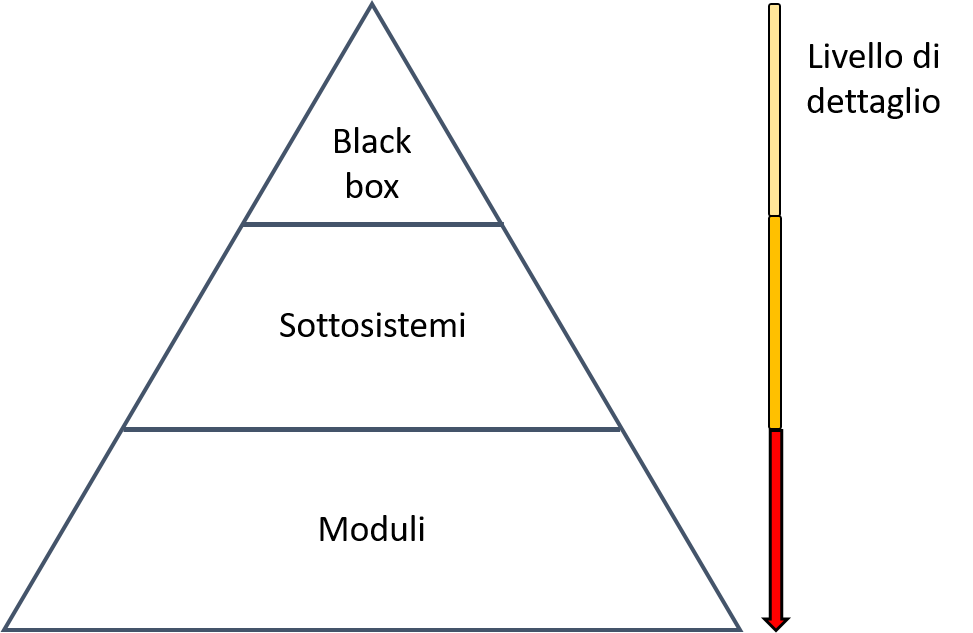
\includegraphics[scale=0.4]{DescrizioneDelSistema/livelli_astrazione.png}
	\caption{Rappresentazione dei livelli d'astrazione utilizzati per descrivere il sistema }
	\label{fig:livelliAstrazione}
\end{figure}
\newpage

\section{Livello black box}
Considerando il sistema in questione come una black box (Fig.\ref{fig:requisitiFunzionali}) e l'infrastruttura di rete in modo astratto, i due macro-requisiti funzionali  sono rispettivamente:
\begin{itemize}
	\item \textbf{R1}: Geolocalizzare l'operatore
	\item \textbf{R2}: Trasmettere messaggi predefiniti come stato della vittima e codici d'emergenza.
\end{itemize}
\begin{figure}[H]
	\centering
	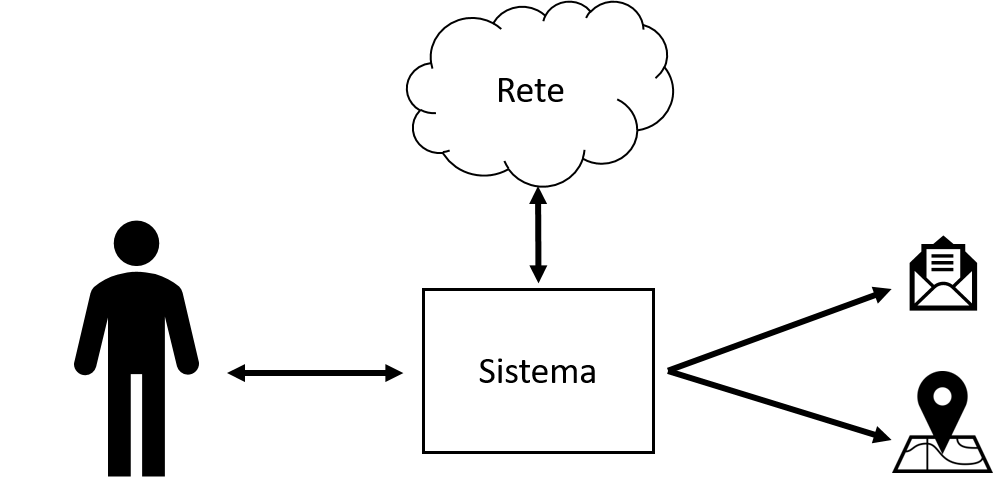
\includegraphics[scale=0.3]{DescrizioneDelSistema/requisitiSistema.png}
	\caption{Rappresentazione del sistema come black box }
	\label{fig:requisitiFunzionali}
\end{figure}
Nelle fasi primordiali del progetto, si è scelto di allocare la maggior parte delle risorse lavorative nel completamento di \textbf{R1} lasciando ad una fase successiva lo sviluppo di \textbf{R2}, per questo motivo d'ora in avanti considereremo come unico requisito la geolocalizzazione dell'operatore. \\
In particolare \textit{R1} può essere suddiviso in due requisiti più specifici:
\begin{itemize}
	\item \textbf{R1.1}: Determinare la posizione di un operatore all'interno della rete
	\item \textbf{R1.2}: Identificare il cammino minimo da un nodo ad un altro
\end{itemize}
Quest'ultimo rappresenta sia la possibilità da parte dell'operatore di eseguire il percorso all'inverso, sia la possibilità che venga raggiunto da una squadra di supporto. A questo punto possiamo scendere al livello d'astrazione successivo (\ref{fig:livelliAstrazione}).
\newpage 

\section{Livello sottosistemi}
Il sistema è stato quindi diviso in due sottosistemi (Fig.\ref{fig:sistema_liv1}) ognuno dei quali con le proprie responsabilità:
\begin{itemize}
	\item \textbf{S1}: ha il compito di ricavare tramite la rete e altri sensori i dati necessari
	\item \textbf{App}: ha il compito di ricevere i dati da S1, elaborarli e infine fornire la posizione dell'operatore all'interno della rete o il percorso verso uno specifico nodo
\end{itemize}

\begin{figure}[H]
	\centering
	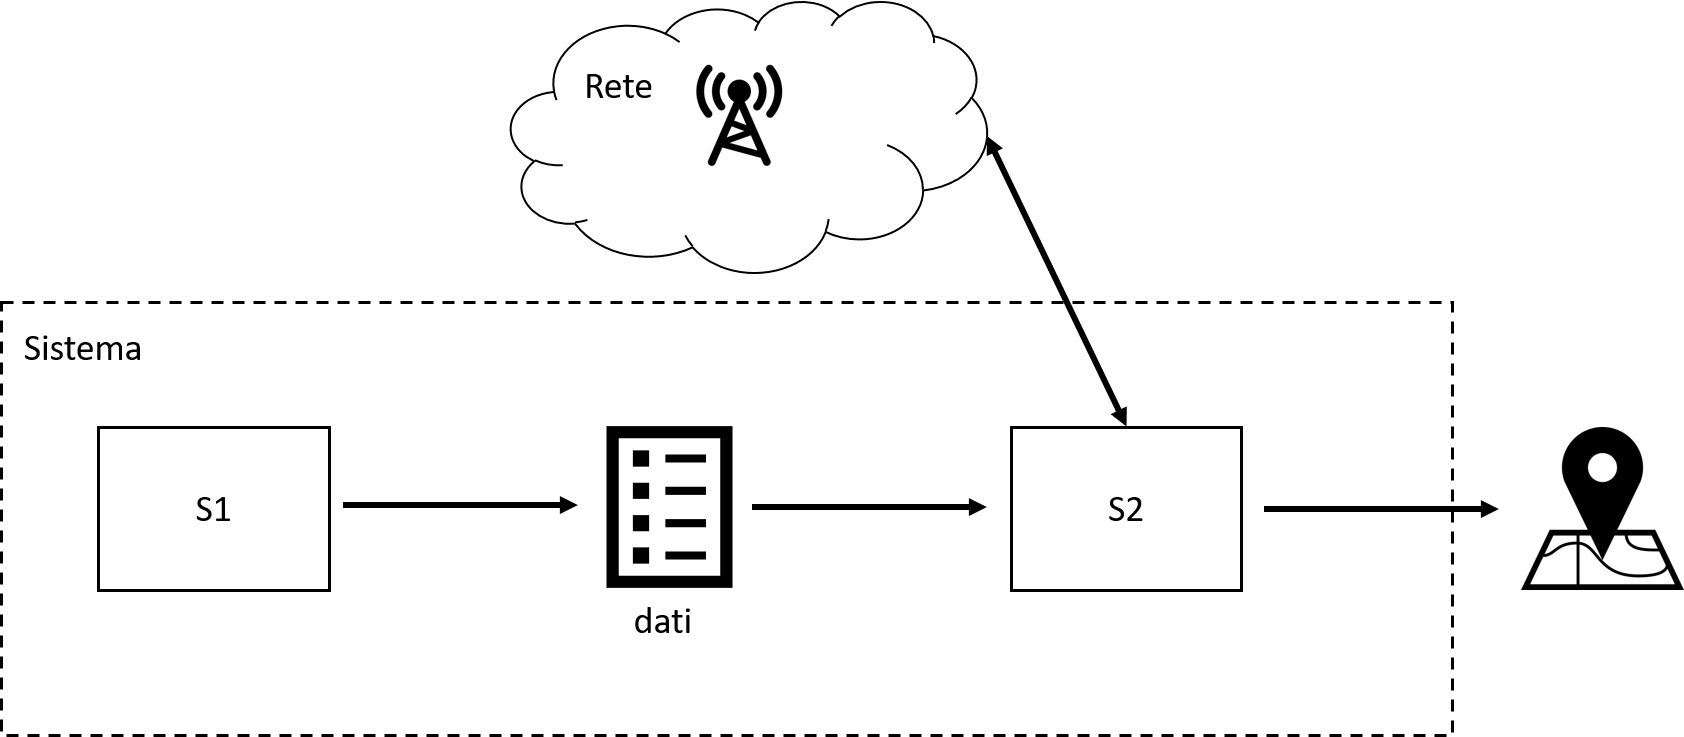
\includegraphics[scale=0.3]{DescrizioneDelSistema/sistema_liv1.png}
	\caption{Rappresentazione del sistema in sottosistemi }
	\label{fig:sistema_liv1}
\end{figure}
L'idea alla base della soluzione del requisito R1 è strettamente legata all'implementazione della rete. Come già accennato nell'introduzione, questa verrà costruita dinamicamente da un'esploratore e man mano che egli avanza verrà ampliata con nuovi nodi. \\
Per mantenere il livello d'astrazione attuale ci basta sapere che le caratteristiche della tecnologia utilizzata nell'implementazione della rete (dettagliata nel capitolo successivo), fa si che le singole celle abbiano un raggio d'azione all'interno del quale il sottosistema \textit{S1} può calcolare la distanza tra l'operatore e il centro della cella stessa. Utilizzando una rete con queste caratteristiche il soddisfacimento di \textit{R1.1} viene quasi del tutto naturale, mentre per quanto riguarda \textit{R1.2} consiste nell'identificare il cammino minimo, problema ben noto in letteratura.\\
Appare evidente a questo punto che il soddisfacimento dei due requisiti si "riduce" alla costruzione dinamica della rete e alla georeferenziazione dei nodi che la compongono.\\
Nel prossimo paragrafo ci porteremo al livello d'astrazione più basso (vedi \ref{fig:livelliAstrazione}) dettagliando i moduli che compongono i due sottosistemi e illustrando come questi intendono risolvere il problema di georeferenziazione appena emerso.


\section{Livello moduli}
La soluzione al problema di georeferenziare la rete si costruisce per iterazione georeferenziando i nodi nel momento in cui vengono aggiunti dall'operatore. Con riferimento all'esempio illustrato precedentemente( vedi Fig.\ref{fig:step1}- Fig.\ref{fig:step6}) consideriamo lo step 2 .\\
Per ipotesi supponiamo che il primo nodo sia già georeferenziato, nel momento in cui risulti essere al limite della line-of-sight e della distanza di sicurezza(20 mt) l'operatore piazzerà il secondo nodo. Per georeferenziarlo (rispetto al primo) abbiamo bisogno di alcune informazioni:
\begin{itemize}
	\item La distanza tra i due nodi
	\item L'angolo tra i due nodi
\end{itemize}

Il vettore distanza può essere ricavato sfruttando la caratteristica tecnologica (vedi rif.tecnologia uwb) della rete da parte del sistema che, è in grado di determinare la distanza tra l'operatore e il nodo all'interno del suo raggio d'azione.\\
Tale informazione non è però sufficiente, infatti ci sono infiniti punti sulla circonferenza con centro nel primo nodo e raggio pari alla distanza. Per poter georeferenziare in modo univoco il secondo nodo abbiamo bisogno di trovare anche l'angolo in riferimento al primo nodo, tale compito non è banale e tanto meno le metodologie univoche e perfette.\\
Per il momento ci basta sapere che l'algoritmo utilizzato nel contesto di questa tesi, approfondito nei capitoli successivi (vedi rif. algoritmo di fusione), esegue un campionamento durante il tragitto tra un nodo e l'altro combinando i dati inerenti alla distanza dell'operatore con quelli relativi agli angoli lungo il percorso.
La figura seguente rappresenta la georeferenziazione del secondo nodo utilizzando soltanto il vettore distanza tra i due nodi.
\begin{figure}[H]
	\centering
	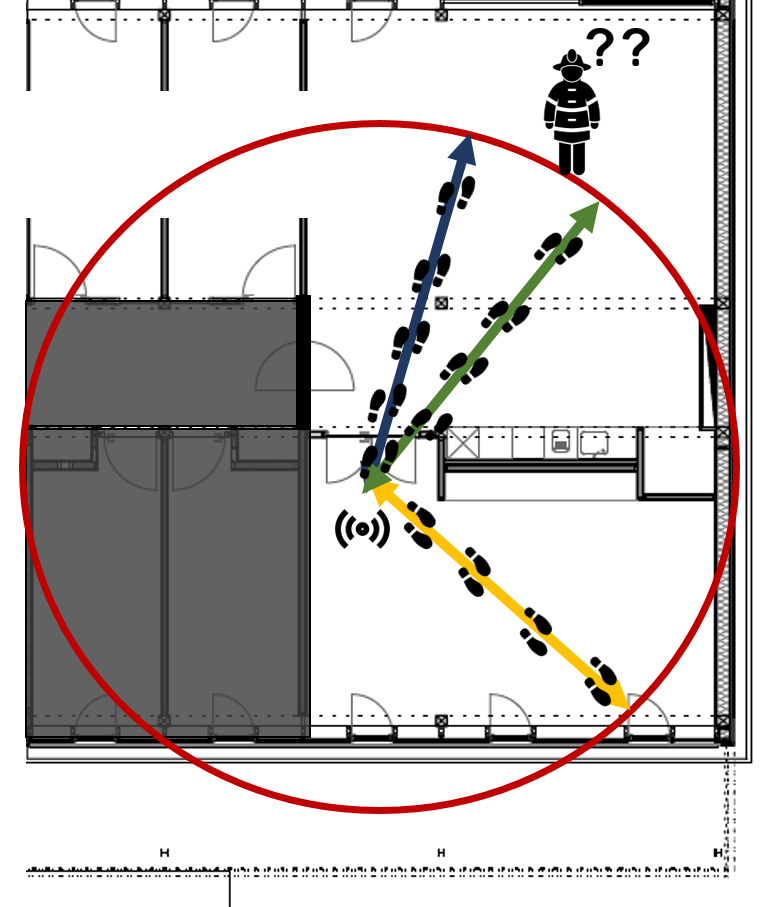
\includegraphics[scale=0.5]{DescrizioneDelSistema/ambiguitDistanza.png}
	\caption{Ambiguità nella georeferenziazione del nodo utilizzando soltanto la distanza con il precedente }
	\label{fig:ambiguitDistanz}
\end{figure}

Nella figura precedente abbiamo graficato solo tre delle possibili infiniti posizioni del secondo nodo utilizzando solo la distanza rilevata. Assumiamo che la direzione corretta sia il punto intersecato dal vettore in blu e la circonferenza, un'ambiguità con il vettore in verde potrebbe essere accettata in quanto pochi metri dalla reale posizione e a causa della mancanza di percorsi verso est, un'ambiguità con il vettore in giallo renderebbe il sistema completamente inutile o peggio disinformante.  

